%!TeX program = xelatex
\documentclass[numberedappendix,twocolumn,twocolappendix,apj]{openjournal}

\usepackage{latexsym}
\usepackage{graphicx}
\usepackage{amssymb}
\usepackage{longtable}
\usepackage{epsf}
\usepackage{amsmath}
\usepackage{graphicx}
%\DeclareMathOperator{\sech}{sech}
\usepackage{hyperref}
\hypersetup{colorlinks=true,linkcolor=blue,citecolor=blue,filecolor=blue,urlcolor=blue}
\usepackage{cleveref}
\usepackage{bm}
\usepackage{lipsum}
\usepackage{enumitem}
\usepackage{newtx}
\usepackage{gensymb}
\usepackage{booktabs}               % better table rules
\usepackage{multirow}
\usepackage{natbib}

%%%%%%%%%%%%%%%%%%%%%%%%%%%%%%%%%%%%%%%%%%%%%%%%%%
\usepackage[table]{xcolor}

\definecolor{hpurple}{HTML}{7E16DF}
\definecolor{hgreen}{HTML}{008F0F}
\definecolor{horange}{HTML}{FFA301}

\newcommand{\todo}[1]{\textcolor{hpurple}{\bfseries [todo: #1]}}
\newcommand{\addcite}{\textcolor{hpurple}{\bfseries [CITE]}}

\newcommand{\dd}{\rm d}
\newcommand{\eg}{\textit{e.g.}}
\newcommand{\ie}{\textit{i.e.}}
\newcommand{\panco}{\texttt{panco2}}
\newcommand{\bibtex}{\textsc{Bib}\!\TeX}

\newcommand{\refeq}[1]{eq.~(\ref{#1})}

\defcitealias{arnaud_universal_2010}{A10}
\newcommand{\aten}{\citetalias{arnaud_universal_2010}}


 %%%%%%%%%%%%%%%%%%%%%%%%%%%%%%%%%%%%%%%%%%%%%%%%%%
\begin{document}

\title{panco2: a Python library to measure intracluster medium pressure profiles from Sunyaev-Zeldovich observations}
\shorttitle{\panco: pressure profiles from tSZ maps}

\author{F. K\'eruzor\'e$^{1,2,\star}$}
\author{F. Mayet$^{2}$}
\author{E. Artis$^{2}$}
\author{L. E. Bleem$^{1}$}
\author{J.-F. Mac\'ias-P\'erez$^{2}$}
\author{M. Mu\~noz-Echeverr\'ia$^{2}$}
\author{L. Perotto$^{2}$}
\author{F. Ruppin$^{3}$}
\author{others?}

\affiliation{
    $^1$High Energy Physics Division, Argonne National Laboratory, 9700 South Cass Avenue, Lemont, IL 60439, USA \\
    $^2$Univ. Grenoble Alpes, CNRS, Grenoble INP, LPSC-IN2P3, 53, avenue des Martyrs, 38000 Grenoble, France \\
    $^3$Univ. Lyon, Univ. Claude Bernard Lyon 1, CNRS/IN2P3, IP2I Lyon, F-69622, Villeurbanne, France
}
\thanks{$^{\star}$E-mail:fkeruzore@anl.gov}

\shortauthors{K\'eruzor\'e et al.}

%%%%%%%%%%%%%%%%%%%%%%%%%%%%%%%%%%%%%%%%%%%%%%%%%%%%%%%%%

\begin{abstract}
    We present \panco, an open-source \texttt{Python} library designed to fit pressure profiles in Sunyaev-Zeldovich maps.
    The fitting procedure is based on forward modeling of the total observed signal, allowing to take into account usual features of millimeter observations, such as beam smearing, data processing filtering, and point source contamination.
    \panco\ offers a large flexibility in the inputs that can be handled and the analysis options, enabling refined analyses and studies of systematic effects.
    We detail the functionalities of the code, the algorithm used to infer pressure profile measurements, and the typical data products.
    We present examples of running sequences, and the validation on simulated inputs.
    The code is available on \href{https://github.com/fkeruzore/panco2}{github}, and comes with an extensive technical documentation to complement this paper.
\end{abstract}

\keywords{Cosmology: large-scale structure of Universe}

\maketitle

\vspace{1cm}

\twocolumngrid

%%%%%%%%%%%%%%%%%%%%%%%%%%%%%%%%%%%%%%%%%%%%%%%%%%
%%%%%%%%%%%%%%%%% BODY OF PAPER %%%%%%%%%%%%%%%%%%

% !TEX root = ./main.tex
\section{Introduction}
\label{sec:intro}

%%% Why clusters are cool
Galaxy clusters are deeply interesting physical objects.
Their abundance in mass and redshift is tightly linked to cosmic evolution, and can therefore be used as a cosmological probe \citep[see \eg][for a review]{allen_cosmological_2011}.
In order to exploit this property, large sky surveys have been used to build catalogs of serendipitously detected clusters at different wavelengths, such as X-rays \citep[\eg][]{liu_erosita_2022}, optical \citep[\eg][]{des_collaboration_dark_2020}, and millimeter-waves \citep[\eg][]{bleem_sptpol_2020}.

%%% Why SZ clusters are the coolest
Among these, one of the wavelengths of choice for the detection of galaxy clusters is the millimeter domain.
Clusters can be observed at such frequencies through the Sunyaev-Zeldovich effect \citep[SZ,][]{sunyaev_observations_1972}, \ie\ the spectral distortion of the cosmic microwave background (CMB) due to the Compton scattering of its photons on the free electrons of gas along the line of sight.
The SZ effect is often separated in different components, depending on the origin of the energy transferred from the electrons; the main components being, by order of decreasing importance, the thermal (tSZ) and kinetic \citep[kSZ,][]{sunyaev_velocity_1980} effects \citep[see][for a recent review of the SZ effects]{mroczkowski_astrophysics_2019}.
Catalogs of clusters detected through their tSZ signal are particularly interesting for cosmological applications, as the amplitude of the tSZ effect does not suffer from cosmological dimming \citep{carlstrom_cosmology_2002}.
As a result, modern millimeter-wave sky surveys have brought us some of the largest and deepest cluster samples to date, with the catalogs built from the Atacama Cosmology Telescope \citep[ACT,][]{hilton_atacama_2021}, the South Pole Telescope \citep[SPT,][]{bleem_sptpol_2020}, and \textit{Planck} \citep{planck_collaboration_planck_2016-2} surveys.

%%% Why do we measure pressure profiles
% tSZ depends on ICM pressure, therefore knowing pressure we know what to look for
The amplitude of the tSZ distortion is directly proportional to the electron pressure in the gaseous intracluster medium (ICM) integrated along the line of sight.
This link between tSZ signal and ICM pressure motivates studies of the pressure distribution in the ICM -- in its simplest form, as a spherically symmetric pressure profile.
For example, matched-filtering cluster detection algorithms may require a prior assumption on the overall shape of the ICM pressure profile \citep[\eg][]{melin_comparison_2012}, in which case a poor knowledge of this property of clusters may lead to a poorly constructed cluster sample.
Similarly, the power spectrum of the tSZ effect on the sky, which can be used to constrain cosmology, strongly relies on an assumption of the pressure profile of clusters, and the recovering of cosmological parameters can be severely affected by its poor knowledge \citep{ruppin_impact_2019}.
% Early studies told us they should all be the same
The mean pressure profile of galaxy clusters has been investigated using different cluster samples over the last decade.
Early works conducted on local, X-ray selected samples, such as \citet[][hereafter \aten]{arnaud_universal_2010}, converged towards a ``universal'' pressure profile, undergoing self-similar redshift and mass evolution \citep[see also \eg][]{battaglia_cluster_2012-1, planck_collaboration_planck_2013}
In these studies, the main determining factor for the shape of the pressure profile of a cluster was its dynamical state, with relaxed clusters exhibiting a steeper pressure profile in their core.
% But hey that was wrong because feedback and stuff
% We'd do simulations but their subgrids need us so the snake is eating its own tail
\textcolor{lightgray}{\lipsum[1]}

%%% How do we measure pressure profiles
The first step in any evaluation of the mean pressure profile of a sample is the extraction of individual profiles from observed data.
% Can be from Xrays
Such measurements can be performed from X-ray cluster observations, using a deprojection of the ICM electron density and temperature \citep[see \eg][for reviews]{bohringer_x-ray_2010, bohringer_x-ray_2013}.
% But that works better for low-z and high-M thingies
Because of cosmological dimming, the X-ray surface brightness measure towards a cluster -- at fixed density -- strongly decreases with redshift, with $S_{\rm X} \propto (1+z)^{-4}$.
As a consequence, X-ray observations of sufficient depth to infer quality measurements of pressure profiles can be prohibitively costly from an observation time perspective for high redshift systems.
% Can be from SZ
Alternatively, one may use tSZ observations of clusters, which do not suffer from this redshift dimming, enabling the detection of more distant objects.
% Need to resolve them but can be done
In particular, high angular resolution millimeter observations of clusters with large aperture telescopes have successfully been used to measure cluster pressure profiles, and are today one of the preferred sources of data for studies of the mean pressure profile of clusters \citep[\eg][]{mayet_cluster_2020, young_mean_2022, sayers_evolution_2022}.

%%% What is this paper
% In this work we present a software to go from SZ map to P(r)
In this paper, we present \panco, a \texttt{Python} library written to perform pressure profile extraction from tSZ observations.
The algorithm is based on forward modeling of the tSZ signal and MCMC sampling, and allows users to account for different features of millimeter-wave observations that may manifest as systematic biases or uncertainties in recovered pressure profiles.
An earlier version of \panco\ was described in \citet{keruzore_panco2_2021}, which offered less flexibility in the analysis, as the only data that could be analyzed was maps from the NIKA2 camera 150~GHz channel \citep{adam_nika2_2018, perotto_calibration_2020}.
This software has already been used for different studies based on NIKA2 data \citep[\eg][]{artis_psz2_2022,munoz-echeverria_multi-probe_2022,munoz-echeverria_lpsz-clash_2022}.
Here, we present a generalization of the code, that makes it able to perform pressure profile extractions from arbitrary data formats.

%%% Outline
The paper is structured as follows.
\textcolor{lightgray}{\lipsum[6]}

Throughout this paper, even though \panco\ can use different cosmologies \todo{this is not true yet}, we assume a flat $\Lambda {\rm CDM}$ model, with $\Omega_{\rm m} = 0.3, \;\Omega_\Lambda = 0.7, \; h = 0.7$.
This cosmology is mainly used to infer angular diameter distances to the cluster being studied from its redshift, in order to accuratrly map sky distances to physical ones.
Quantities with a $500$ subscript refer to the properties of a cluster within its characteristic radius $R_{500}$, corresponding to the radius of a sphere around the center of the cluster in which the mean matter density is $500$ times the critical density of the Universe at the cluster's redshift.

% !TEX root = ./main.tex
% ========================================================================== %
\section{Algorithm} \label{sec:algo}

The goal of \panco\ is to infer a measurement of a pressure profile and of its confidence intervals from the SZ map of a cluster.
The overall workflow implemented in \panco\ to perform this measurement is presented in Figure~\ref{fig:workflow}.
It is based on the forward modeling of the SZ map and on Monte-Carlo Markov Chain (MCMC) sampling of the probability distribution for the pressure profile parameters given the input data.
In this section, we detail each step of the analysis, as well as the inputs to be given to \panco\ and the results it produces.

\begin{figure*}[htp]
    \centering
    \includegraphics[width=.9\linewidth]{Figures/workflow.drawio.pdf}
    \caption{
        Schematic workflow of the \panco\ algorithm, from its inputs (blue), to the forward modeling and MCMC sampling (purple), and results (red).
        Required and optional inputs are denoted with boldface and italic fonts, respectively.
    }
    \label{fig:workflow}
\end{figure*}

% -------------------------------------------------------------------------- %
\subsection{Data inputs} \label{sec:algo:inputs}

The main input of \panco\ is a mapping of a patch of the sky containing SZ signal.
The code uses the FITS standard \citep{wells_fits_1981} to correctly map sky coordinates to pixels using the flat-sky approximation.
The map to be fitted must therefore be contained within a FITS file, that must include the following ingredients:

\begin{itemize}[leftmargin=*]
    \item An extension in which the data is the SZ map to be fitted, and the header includes the World Coordinate System (WCS) used to create the map;
    \item An extension in which the data represent an estimate of the expected root mean squared (RMS) error for each pixel of the data map.
\end{itemize}

Such a file constitutes the minimum data input for \panco\ to proceed fitting a pressure profile.
Using these inputs, the user may choose to only use a square portion of the map, by specifying the sky coordinates of its center and its side.

Additional inputs can be provided to account for various data features.
\paragraph{Beam smearing} the user may provide the width of a Gaussian function to account for point spread function (PSF, hereafter referred to as ``beam'') filtering (see \S\ref{sec:algo:fwdmod});
\paragraph{Transfer function} Fourier filtering due to data processing and/or scanning strategy can be accounted for in the analysis (see \S\ref{sec:algo:fwdmod});
\paragraph{Point source contamination} the position on the sky of point sources, as well as their fluxes and uncertainties, can be used to account for the contamination and marginalize over its amplitude (see \S\ref{sec:algo:fwdmod});
\paragraph{Correlated noise} the covariance matrix between the noise of pixels in the map can be provided (see \S\ref{sec:algo:likelihood}).

% -------------------------------------------------------------------------- %
\subsection{Pressure profile model} \label{sec:algo:press}

The electron pressure distribution in the ICM is modeled in \panco\ as a radial pressure profile, implying spherical symmetry of the ICM.
The most widely used parametrization for ICM pressure profiles, called the generalized Navarro-Frenk-White model \citep[gNFW,][]{zhao_analytical_1996, nagai_effects_2007}, is known to have several shortcomings.
In particular, the very self-constrained shape of the functional form of the profile and the important correlations in the parameter space make model fitting complex, and the recovered parameter values hard to interpret \citep[see \eg][]{nagai_effects_2007, battaglia_cluster_2012-1, sayers_evolution_2022}.

In order to try to circumvent these issues, \panco\ uses a more flexible parametrization of the pressure profile, in which the pressure distribution is modeled as a power law evolution in concentric spherical shells.
In this modeling, the model parameters are the values $P_i$ of the pressure profile at predefined radii from the cluster center $R_i$, with a power law interpolation between the radii\footnote{Several papers in the literature have dubbed this modeling a ``non-parametric'' approach; as this may induce confusion, since the model is parametric, we will refrain from using this term, and refer to our model as ``radially binned''.}:
\begin{equation}
    \label{eq:algo:pressure_profile}
    P(r \in [R_i, R_{i+1}[) = P_i \left(r / R_i\right)^{-\alpha_i},
\end{equation}
where $\alpha_i = - \log(P_{i+1} / P_i) / \log(R_{i+1} / R_i)$. \\
Outside of the radial bins, the pressure profile is extrapolated using the power-law evolution of the first (last) bin.
In addition to being more flexible and having generally lesser correlations in the parameter space, this parametrization can be integrated along a line of sight analytically through Abell transform, by following \eg\ \citet{romero_multi-instrument_2018}.

The main downside to this pressure profile modeling lies in the need to specify the radii $R_i$ used in \refeq{eq:algo:pressure_profile} \textit{a priori} when performing a fit.
There is no obvious, fail-safe way to define this radial binning.
A user may choose a binning motivated by the data coverage (\eg\ with radii that, projected on the sky plane, are separated the beam of the instrument used to build the map); but looking at the same data, another user may be motivated by sample studies over several cluster, and wish to define a binning in units of a characteristic radius of the cluster (\eg\ $R_{500}$).
As a result, model dependence may arise in the results produced by \panco.
This point will be addressed in \S\ref{sec:end}.

% -------------------------------------------------------------------------- %
\subsection{Forward modeling: from pressure profile to SZ map} \label{sec:algo:fwdmod}

\begin{figure}
    \centering
    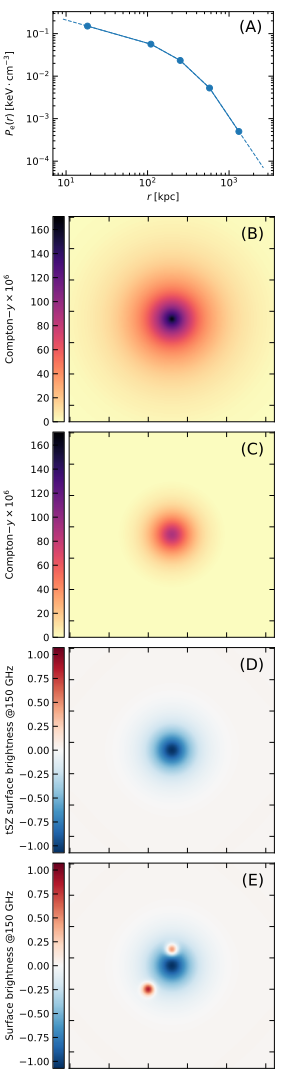
\includegraphics[height=0.933\textheight]{Figures/fwmod.pdf}
    \caption{
        Illustration of the forward modeling procedure.
        The pressure profile (A) is integrated along the line of sight to create a Compton$-y$ map (B), which is filtered (C) and converted (D) to be realistically comparable to the observed data.
        If point source contamination information is passed, point source models can be added to the map (E).
    }
    \label{fig:fwmod}
\end{figure}

The approach used by \panco\ to fit pressure profiles on SZ maps is forward modeling.
In that framework, a pressure profile model -- determined by \refeq{eq:algo:pressure_profile} -- is used to generate a map that can be compared to data.
This approach has been vastly used in the estimation of pressure profiles from tSZ maps, especially in the context of resolved follow-up of galaxy clusters with \eg\ NIKA2 \citep[\eg][]{munoz-echeverria_multi-probe_2022,keruzore_exploiting_2020}, MUSTANG(2) \citep[\eg][]{romero_galaxy_2017,romero_pressure_2020}, Bolocam \citep[\eg][]{sayers_evolution_2022}, or ALMA \citep[\eg][]{di_mascolo_joint_2019}.
This section details the different steps used in that process, which is ilustrated in figure~\ref{fig:fwmod}.

\paragraph{Line of sight integration}

The amplitude of the tSZ effect in a direction $\theta$ on the sky is named the Compton parameter $y$, and is proportional to the integral along of the electron pressure along the line of sight (LoS):
\begin{equation}
    \label{eq:algo_ysz}
    y(\theta) = \frac{\sigma_\textsc{t}}{m_{\rm e}c^2} \int_{\rm LoS(\theta)} P_{\rm e} \; \dd l,
\end{equation}
where $\sigma_\textsc{t}$ is the Thompson cross-section, and $m_{\rm e} c^2$ is the electron resting energy. \\
In \panco, we perform this integration analytically, by following the derivation presented in Appendix A of \citet{romero_multi-instrument_2018}, using the spherically symmetric case (in the notation of \citeauthor{romero_multi-instrument_2018}, $a_i = b_i = c_i = 1 \; \forall \; i$).
This allows us, for any given pressure profile, to create a Compton parameter map in the same coordinate system as the data, \ie\ an estimate of the value of $y$ for each pixel in the map.

\paragraph{Conversion and zero level}

Depending on the data product available, and on the convention used in the raw data processing software employed to create these data products, tSZ maps can have a variety of units (\eg\ surface brightness, CMB temperature fluctuation).
These units can usually be converted to Compton$-y$ through a scalar conversion coefficient, $C_{\rm conv}$, which can depend on many different quantities that may be difficult to estimate, or even fluctuate during observations, such as instrumental bandpasses, weather conditions, instrumental calibration, or even temperature of the ICM through relativistic corrections to the tSZ effect \citep{mroczkowski_astrophysics_2019}.
As a result, the conversion coefficient is affected by an uncertainty.
In \panco, this coefficient is treated as a parameter in the model, for which a prior distribution needs to be specified (see \S\ref{sec:algo:mcmc}), allowing to propagate the uncertainty on the conversion of the map to the pressure profile estimate.
This means that a vector in the parameter space will contain a value of a conversion coefficient, which \panco\ multiplies the model $y-$map by to get a map in the same units as the input data.
In case the input data is already in units of Compton$-y$, this coefficient may still be used to propagate multiplicative calibration uncertainty by centering the prior distribution on 1.
In addition, in order to enable taking into account possible large-scale residual noise, a zero-level offset can be added to the map, and marginalized over.

\paragraph{Filtering}

The tSZ maps constructed by any instrument are affected by different types of filtering.
The instrumental PSF acts as a filter that smooths the data by suppressing signal at small scales.
In its forward modeling approach, \panco\ is able to take into account this filtering by convolving the model $y-$map with a 2D Gaussian filter, the width of which can be specified by the user.

In addition, during the data reduction process used to create tSZ maps from raw data, filtering can occur, often suppressing signal at large angular scales.
This filtering is usually accounted for through a transfer function, quantifying the signal filtering in the Fourier space, and evaluated during the data processing.
\panco\ can account for this effect by filtering the map with a transfer function provided by the user.
Two different types of transfer functions can be provided:
\begin{itemize}[leftmargin=*]
    \item a 1D transfer function: assuming that the filtering is isotropic, \panco\ can convolve model maps with a 1D kernel specified by the user as angular frequencies $k$ and their associated filtering ${\rm TF}(k)$;
    \item a 2D transfer function: if the filtering on the sky cannot be assumed to be isotropic, the user may specify 2D angular scales $(k_x, k_y)$ and their corresponding filter ${\rm TF}(k_x, k_y)$.
\end{itemize}
A thorough discussion of the impact of choosing a 1D or 2D transfer function -- in the case of NIKA2 data, in which the filtering is mildly anisotropic -- can be found in \citet{munoz-echeverria_multi-probe_2022}.

\paragraph{Point source contamination}

After applying the different filters, the \panco\ model map is a map of the tSZ signal, in the unit and mapping as the input data, and having been affected by the same signal filtering.
It is therefore comparable to the tSZ signal in the input map.
But millimeter-wave maps of cluster regions may also include astrophysical signal from other sources.
In particular, signal from millimeter-emitting galaxies can often be found in such maps.
These galaxies can be foreground, background, or cluster members, and their emission can be thermal (in the case of dusty star-forming galaxies), or synchrotron (for radio-loud AGN).
In any case, this signal manifests as a contamination for tSZ science, and must be accounted for in data analysis, lest the recovered pressure profile be biased.

In its forward modeling approach, \panco\ uses the methodology described in \eg\ \citet{keruzore_exploiting_2020}, in which point source models may be added to the tSZ model map in order to model the total signal in the map.
The spatial model of each source is given by the instrumental PSF, and their fluxes are treated as model parameters, with priors specified by the user (see \S\ref{sec:algo:mcmc}).
If the flux of a source is well known from external data, this prior will be tight, and serve as a propagation of its uncertainty to the recovered pressure profile.
Otherwise, if a source is known to be present but little is known about its flux, large priors can be used, in which case \panco\ will constrain the sum of the tSZ signal and the point source flux\footnote{\panco\ is able to constrain the sum of the two because of the different spatial distribution of the tSZ and point source fluxes.}.
To account for point source contamination in the analysis, the user must therefore provide \panco\ with a position (in sky coordinates) and a probability distribution for the flux (in input map units) for each of the sources considered.

% -------------------------------------------------------------------------- %
\subsection{Likelihood} \label{sec:algo:likelihood}

The process described in \S\ref{sec:algo:fwdmod} allows \panco\ to compute a model map that is comparable to the input data from any position in the parameter space.
To summarize, a vector in this parameter space, $\vartheta$, has the following components:
\begin{itemize}[leftmargin=*]
    \item $P_0, \dots P_n$: the value of the pressure profile at each predefined radius $R_0, \dots R_n$ ; \\
    \item $C_{\rm conv}$: the conversion coefficient from Compton$-y$ to input map units;
    \item $Z$: a zero-level for the map;
    \item If provided, $F_0, \dots F_m$: the fluxes of point sources in the map, in input map units.
\end{itemize}

The comparison between the model map and the input data is performed through a Gaussian likelihood function:
\begin{align}
    \nonumber -2 \log \mathcal{L}(\vartheta) & \equiv -2 \log p(D | \vartheta) + {\rm cst.} \\
        & = \left[D - M(\vartheta)\right]^{\rm T} \mathbf{C}^{-1} \left[D - M(\vartheta)\right],
    \label{eq:algo:likelihood}
\end{align}
where $D$ is the input map, $M(\vartheta)$ is the model map computed from the position in parameter space $\vartheta$, and $\mathbf{C}$ is the noise covariance matrix. \\
If the noise in the map can be considered white, the noise values in the map pixels are uncorrelated, and $\mathbf{C}$ becomes diagonal.
In that case, in order to reduce the computation time needed, the likelihood is rewritten as:
\begin{equation}
    \label{}
    -2 \log \mathcal{L}(\vartheta) = \sum_i \left( \frac{D_i - M_i(\vartheta)}{\Sigma_i} \right)^2,
\end{equation}
where the sum runs over all pixels $i$ in the map, and $\Sigma$ is the noise RMS map.

% -------------------------------------------------------------------------- %
\subsection{Posterior distribution and MCMC sampling} \label{sec:algo:mcmc}

\panco\ performs the extraction of pressure profile from tSZ data using Bayesian MCMC.
In that framework, a prior probability distribution for the parameters, $p(\vartheta)$, must be multipled to the likelihood function of \refeq{eq:algo:likelihood} to obtain a posterior distribution for the parameters given the data: $p(\vartheta | D) \propto p(D | \vartheta) \, p(\vartheta)$.
In \panco, the prior distributions for the different model parameters are considered uncorrelated, meaning the prior distribution is the product of the individual priors on parameters:
\begin{equation}
    \label{}
    p(\vartheta) = \prod_i p(\vartheta_i),
\end{equation}
where the product runs over all individual parameters $i$. \\
The prior on each parameter is to be specified by the user, using the large variety of distributions available in the \texttt{scipy.stats}\footnote{\url{https://docs.scipy.org/doc/scipy/reference/stats.html}} module \citep{virtanen_scipy_2020}.

The resulting posterior distribution, $p(\vartheta | D)$, is then sampled using MCMC.
More specifically, we use the affine-invariant ensemble sampling implementation of the \texttt{emcee} library \cite{foreman-mackey_emcee_2019}.
Convergence of the walkers is monitored at regular intervals based on the autocorrelation length of the chains, using the following algorithm.
Every $n_{\rm check}$ steps (\ie\ accepted positions in the parameter space), the integrated autocorrelation length $\tau_j$ of each chain $j$ is computed, as well as the average autocorrelation over all chains, $\tau = \left< \tau_j \right>$.
Convergence is accepted if both of the two following criteria are met:
\begin{enumerate}[leftmargin=*]
    \item The current length of the chains is longer than $n_{\rm auto} \times \tau$;
    \item The mean autocorrelation has changed by less than $\Delta\tau_{\rm max}$ in the last two evaluations.
\end{enumerate}
The values of $n_{\rm auto}$ and $\Delta\tau_{\rm max}$ are parameters of \panco, that need to be specified by the user.
Likewise, the user needs to provide a maximum chain length at which the sampling should stop if convergence was never reached.

% -------------------------------------------------------------------------- %
\subsection{Chains cleaning and exploitation} \label{sec:algo:outputs}

Once MCMC convergence has been reached, \panco\ stores the full sampling of the posterior distribution, \ie\ all of the accepted positions in the parameter space and their associated log-likelihood and log-posterior values.
The raw chains can then be loaded and cleaned as follows:
\begin{enumerate}[leftmargin=*]
    \item Remove the first $n_{\rm burn}$ samples as a burn-in length;
    \item Thin the chains by discarding $(n_{\rm discard} - 1) / n_{\rm discard}$ samples, \ie\ only keeping one sample every $n_{\rm discard}$ steps;
    \item Discard the chains that are poorly mixed, \ie\ systematically outside of the $[q_{\rm extr}, 1 - q_{\rm extr}]$ quantiles of the sampled posterior.
\end{enumerate}
Again, the values of $n_{\rm burn}$, $n_{\rm discard}$ and $q_{\rm extr}$ are parameters of the analysis, that must be user-provided.

The cleaned chains can then be expressed in the pressure profile space.
To do so, \refeq{eq:algo:pressure_profile} is used to compute a profile for each position in the parameter space, over a radial range specified by the user.
These profiles may then be saved for future analyses.

The Markov chains, in the parameter space and in the pressure profile space, constitute the main data product of \panco.
Several figures can be produced for a visual representation of the results.
They are all presented in the technical documentation \todo{add link}; we give here a brief description of these figures.

\paragraph{Posterior distribution}
Several functions are available to produce figures showing properties of the Markov chains and the posterior distribution they sample, using the \texttt{ChainConsumer} library \citep{hinton_chainconsumer_2016}:
\begin{itemize}[leftmargin=*]
    \item Walks plot, \ie\ the evolution of the positions in the parameter space with the number of steps for each parameter;
    \item Corner plot, \ie\ a figure showing the marginalized posterior for all individual parameters and sets of two parameters.
        The prior distribution can be overplotted for comparison purposes;
    \item Plot of the correlation and covariance matrices of the different parameters.
\end{itemize}

\paragraph{Data -- Model -- Residuals}
Two figures can be produced to illustrate the quality of the fit.
They both consist in comparing the input data, the best-fitting model, and the residuals (\ie\ the difference between input data and best-fitting model).
These can be plotted in 2D, by showing the three maps side-by-side (see figure~\ref{fig:valid:dmr_2d}), or in 1D, by showing the radial profiles of each of these maps in the same graph (see the left panels of figure~\ref{fig:valid:profiles}).
Goodness of fit can be judged in both representations by lack of significant structure in the residuals.

\paragraph{Pressure profile}
In addition, a plot of the median of these profiles, as well as confidence intervals chosen as their 16th and 84th percentiles, can be produced (see the right panels of figure~\ref{fig:valid:profiles}).

% ========================================================================== %
\section{Validation on simulations} \label{sec:simu}

In order to ensure that \panco\ is able to recover accurate pressure profile measurements, we test it on simulated inputs.
In this section, we detail this validation process, from the creation of the dataset to the results produces by \panco.
For reproducibility purposes, the datasets created and used for this analysis are made public with the software.

% -------------------------------------------------------------------------- %
\subsection{Sample selection}

The goal of the validation is to ensure that \panco\ is able to recover accurate pressure profiles from different types of data.
To that end, we seek to create realistic synthetic cluster maps from three instruments: the \textit{Planck} satellite, the South Pole Telescope (SPT), and the NIKA2 camera at the IRAM 30 m telescope.
The choice of these three instruments is motivated by their vastly different angular resolutions: the Compton$-y$ maps built from \textit{Planck} and SPT data have angular resolutions (expressed as the full width at half maximum, or FWHM) of 10 and 1.25 arcmin, respectively \citep{planck_collaboration_planck_2016, bleem_cmbksz_2022}, and the beam of the NIKA2 camera 150 GHz band -- used for tSZ mapping -- has an FWHM of 18 arcsec \citep{perotto_calibration_2020}.

We choose to create SZ maps for three clusters, labeled (C1, C2, C3), covering different regions of the mass-redshift plane:
\begin{alignat}{2}
    \nonumber {\rm C1}:\; & z=0.05,\ & M_{500} = 9 \times 10^{14} \ M_\odot ;\\
    \nonumber {\rm C2}:\; & z=0.5,\  & M_{500} = 5 \times 10^{14} \ M_\odot ;\\
              {\rm C3}:\; & z=1,\    & M_{500} = 3 \times 10^{14} \ M_\odot,
\end{alignat}
These mock clusters are shown as red stars in figure~\ref{fig:valid:sample}.
The top panel shows their positions in the mass-redshift plane, indicating that C1, C2 and C3 are realistic detections for the \textit{Planck}, SPT, and ACT tSZ surveys, respectively.
Tbe bottom panel of figure~\ref{fig:valid:sample} places the clusters in the angular diameter-redshift plane, showing that C1 can be resolved in \textit{Planck}, SPT, and NIKA2 tSZ maps, while C2 and C3 are too small to be resolved by \textit{Planck}.

\begin{figure}[tp]
    \centering
    \includegraphics[width=\linewidth]{Figures/validation_sample.pdf}
    \caption{
        Validation cluster sample (red stars) in the mass-redshift plane (\textit{top panel}) and in the angular size-redshift plane (\textit{bottom panel}).
        For illustration, the top panel includes clusters detected in recent tSZ surveys: \textit{Planck} \citep{planck_collaboration_planck_2016-2}, ACT \citep{hilton_atacama_2021}, and SPT \citep{bleem_sptpol_2020,bleem_galaxy_2015}.
        Note that the redshift axis is truncated to $z<1.6$, therefore not showing all clusters in these samples.
        Colored lines in the bottom panel show the evolution of the angular $2\times\theta_{500}$ with redshift for clusters of different masses.
        The angular resolutions of the \textit{Planck} and SPT $y-$maps, as well as that of the NIKA2 camera at 150~GHz, are represented as dotted horizontal lines.
    }
    \label{fig:valid:sample}
\end{figure}

% -------------------------------------------------------------------------- %
\subsection{Data generation}

% -------------------------------------------------------------------------- %
\subsection{Pressure profile fitting}

% -------------------------------------------------------------------------- %
\subsection{Results}

% !TEX root = ./main.tex
% ========================================================================== %
\section{Conclusions and discussion} \label{sec:end}

This paper presents the release of \panco, a software enabling its users to perform pressure profile extraction from a tSZ map.
We have presented the main features of the software, based on forward modeling MCMC of the tSZ signal with a radially-binned pressure profile.
We have presented the variety of observational systematics that can be incorporated in the modeling in order to account for the known features of millimeter-wave observations.
In section \S\ref{sec:simu}, we have shown that \panco\ could retrieve unbiased pressure profile estimates from \textit{Planck}-like, SPT-like, and NIKA2-like data, effectively covering a range of angular resolutions from $18''$ to $10'$.
The software is made public, along with a detailed documentation providing deeper technical insights on the code and its usage.

% -------------------------------------------------------------------------- %
\subsection{Products released}

The entirety of the \panco\ software is made available as a github repository\footnote{\url{https://github.com/fkeruzore/panco2}}.
That same repository also includes the data generated for the validation described in \S\ref{sec:simu}, along with the products of said validation (\ie\ the Markov chains and the running sequences used for each dataset).
Alternatively, \panco\ can be installed through \texttt{pip} as follows \todo{not true yet}:
\begin{verbatim}
    $ pip install panco2
\end{verbatim}

In addition, \panco\ is also accompanied by an online technical documentation \todo{url}.
It includes detailed explanations of the technical aspects of the code, as well as a description of the inputs and outputs of \panco's different functions.
The documentation also gives examples of analyses that can be performed with \panco\ beyond the ones presented in the validation.

% -------------------------------------------------------------------------- %
\subsection{Possible future improvements}

This release of \panco\ allows a user to perform the fit of a radially binned pressure profile model on a tSZ map.
Several additional features can be thought of to offer more flexibility in this kind of analysis.
Here, we offer a non-exhaustive list of possible such extensions.
We strongly emphasize that this list should \textit{not} be interpreted as a list of features currently in development by the authors, but instead as a collection of possible avenues to explore.

\paragraph{Joint analysis of several tSZ maps} % ........................... %
We have shown in \S\ref{sec:simu} that \panco\ could recover pressure profiles from tSZ observations with different kinds of instruments -- namely, we have tested \textit{Planck}-, SPT-, and NIKA2-like mappings.
But our analysis treated all of these datasets separately.
For clusters with available data from several instruments, there may be interesting information to be extracted from the joint analysis of several maps \citep[see \eg][]{ruppin_first_2018, romero_multi-instrument_2018}.

\paragraph{Different profile parametrizations} % ........................... %
As discussed in \S\ref{sec:algo:press}, many studies of pressure profiles from tSZ (or X-rays) observations use the gNFW profile.
Even though our radially-binned parametrization offers more flexibility and circumvents the known problems of the usual gNFW parametrization, one may be interested in using other functional forms of pressure profile.
For example, the rewriting of the gNFW model from \citet{battaglia_cluster_2012-1} \citep[see also \eg][]{sayers_evolution_2022} offers a way to constrain the same functional form, but minimizing the correlations in the parameter space.
Even though it is still possible to use a radially-binned profile and to fit any other functional form on the pressure bins \textit{a posteriori} \citep[see \eg][]{munoz-echeverria_multi-probe_2022}, one may want to directly fit said parametrization to the data, which is currently not supported.

\paragraph{Non-spherical pressure models} % ................................ %
Galaxy clusters are well known to not be perfectly spherical structures.
Consequently, fitting a spherically-symmetric pressure distribution misses some information potentially contained in tSZ maps.
For examples, clusters can be aspherical because they are an ongoing merger of two substructures.
Observations of such systems can give precious insights on the dynamics of cluster mergers, and therefore on the physics of large-scale structure formation.
Additionally, non-merging clusters may be aspherical because of their connection to the cosmic web, which can provide interesting insights on cosmic filaments.
Therefore, the possibility to fit pressure distributions beyond spherical symmetry is interesting.
Depending on the morphology of the system, this may be done by fitting for an ellipsoidal pressure distribution \citep[\eg][]{sarazin_deep_2016}, or the sum of the contributions of two (possibly spherical) halos \citep[\eg][]{artis_psz2_2022}.
These possibilities are not implemented in \panco, but might be an interesting extension.

\paragraph{Joint tSZ--X-ray analysis} % .................................... %
The \textit{bremsstrahlung} of hot electrons makes the ICM emit in the X-ray domain \citep[see \eg][for reviews]{bohringer_x-ray_2010, bohringer_x-ray_2013}.
This radiation carries information on the ICM that is very complementary to that offered by tSZ observations.
Namely, similarly to how tSZ signal is linked to the electron pressure in the ICM -- as seen in eq.~(\ref{eq:algo_ysz}) -- X-ray emission is linked to its (squared) electron density.
Moreover, for sufficiently deep observations, X-ray data can also be used to study the spectral distribution of the detected photons, enabling measurements of the ICM electron temperature.
The combination of X-ray and tSZ observations of clusters therefore offers a way to finely characterize ICM thermodynamics.
This complementarity can be exploited \textit{a posteriori}, \eg\ by combining results from \panco\ with density and temperature profiles obtained independently of X-ray data \citep[\eg][]{keruzore_exploiting_2020}, or through a joint fit of the thermodynamic properties \citep[\eg][]{castagna_joxsz_2020-1}.
The possibility of joint tSZ--X-ray fits could be added to \panco\ to take further advantage of this complementarity.

% -------------------------------------------------------------------------- %
\subsection{Recommendations to users}

\todo{this is a terrible section title, please help}

As discussed in \S\ref{sec:algo:press}, the pressure model fitted on the data requires the user to define a set of radii used as nodes for the power-law interpolation of the profile.
The choice of these radii is far from straightforward, as it depends on the angular scales present in the data to be fitted, as well as on the scientific goals of the analysis.
This is the main downside of the radially binned model used in \panco, as the radii chosen may have a significant impact on the analysis results.
The model dependence of products derived from radially-binned pressure profiles has been discussed by \citet{munoz-echeverria_multi-probe_2022}, who show that hydrostatic mass estimates, linked to the first derivative of the pressure profile, are particularly affected.

In order to try to circumvent this shortcoming, we strongly advise \panco\ users to be cautious about their choice of binning, and, when possible, to try different binnings.
We have implemented functions in \panco\ that allow users to easily simulate a mock tSZ map mimicking the data to be fitted.
We encourage users to use this functionality to create such datasets and try out their choices of radial binning on these.
Similarly to the validation presented in \S\ref{sec:simu:results}, the comparison of the pressure profile reconstructed with the one used to generate the map will provide insights on how well adapted a choice of radial binning is to a dataset.
How to perform such an analysis is presented in the technical documentation, at \todo{url}.



% !TEX root = ./main.tex
\section*{Acknowledgements}

\small
The development of \panco\ comes after many years of work on pressure profile fitting codes within the NIKA2 collaboration, for which we acknowledge major contributions by R. Adam and C. E. Romero.
Argonne National Laboratory’s work was supported by the U.S. Department of Energy, Office of Science, Office of High Energy Physics, under contract DE-AC02- 06CH11357.
\normalsize


%%%%%%%%%%%%%%%%%%%%%%%%%%%%%%%%%%%%%%%%%%%%%%%%%%
%%%%%%%%%%%%%%%%%%%% REFERENCES %%%%%%%%%%%%%%%%%%

\bibliographystyle{aasjournal}
\bibliography{panco2}

%%%%%%%%%%%%%%%%%%%% APPENDICES %%%%%%%%%%%%%%%%%%

\appendix

% !TEX root = ./main.tex
\section{some appendix?}
\label{sec:app:1}

\textcolor{lightgray}{\lipsum[1]}


%%%%%%%%%%%%%%%%%%%%%%%%%%%%%%%%%%%%%%%%%%%%%%%%%%

% Don't change these lines
%\bsp	% typesetting comment
%\label{lastpage}
\end{document}
